\question{}

เราต้องการแขวนกรอบรูปอันหนึ่งด้วยเชือก 1 เส้นที่ร้อยจากขอบซ้ายของรูป คล้องเหนือหมุดบนกำแพงบางอัน 
แล้วมาร้อยเชื่อมกับขอบขวาของรูป

\marginnote[\baselineskip]{%
    \centering

    \noindent
    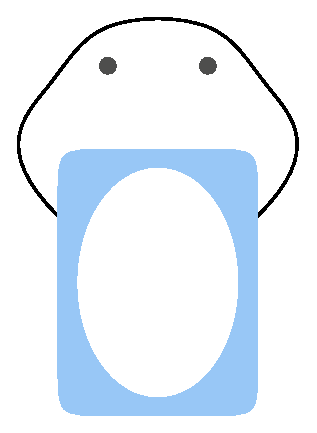
\includegraphics[scale=0.5]{figures/ponder_national_picturehang_01.eps}
    \hfill
    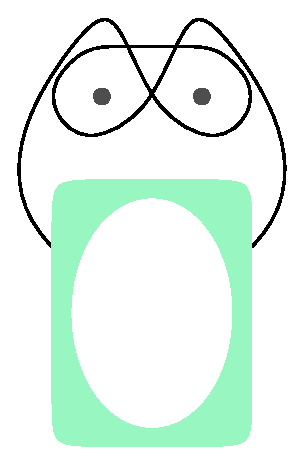
\includegraphics[scale=0.5]{figures/ponder_national_picturehang_02.eps}
    
    \bigskip\noindent
    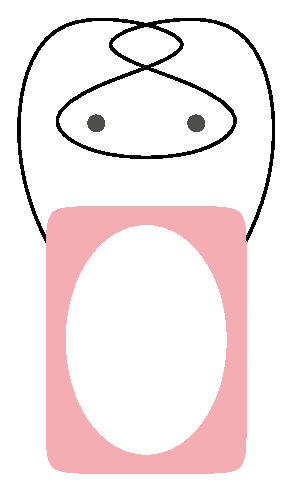
\includegraphics[scale=0.5]{figures/ponder_national_picturehang_03.eps}
    \hfill
    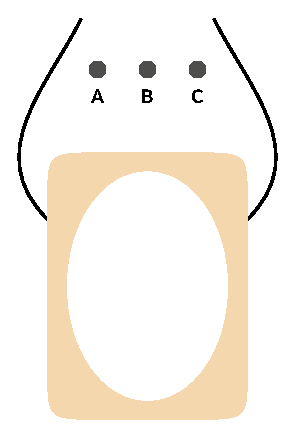
\includegraphics[scale=0.5]{figures/ponder_national_picturehang_04.eps}
}

\medskip\noindent
\textbf{\uline{ตัวอย่าง}\; หมุด 2 ตัว} ---
สมมติว่าเราเลือกที่จะแขวนรูปโดยการร้อยเชือกกับหมุด 2 ตัวในรูปแบบต่าง ๆ ดังนี้
\begin{itemize}[before*=\small]
\item \textbf{รูปสีฟ้า:} หากเราแขวนรูปด้วยวิธีปกติ (ดังรูปสีฟ้า) เราพบว่าหากหมุด\uline{ตัวใดตัวหนึ่ง}ถูกดึงออกไป 
    หมุดอีกตัวหนึ่งจะยังสามารถรั้งกรอบภาพ\uline{ไม่ให้ตก}ตามแรงโน้มถ่วงได้
\item \textbf{รูปสีเขียว:} แต่หากเราแขวนอีกแบบหนึ่ง (ดังรูปสีเขียว) เราพบว่ากรอบภาพจะยังคงแขวนได้เช่นกัน
    แต่หากหมุดตัวใดตัวหนึ่งถูกดึงออกไป กรอบภาพจะ\uline{หลุดลงมาทันที}แม้ว่าหมุดอีกตัวจะยังยึดกำแพงอยู่ก็ตาม
\end{itemize}

\noindent
\textbf{\uline{โจทย์}\; หมุด 3 ตัว} ---
หากเรามีหมุดสามอัน คือ A, B, C เรียงจากซ้ายไปขวา (ดู\textbf{รูปสีส้ม}ประกอบ) 
เราต้องการร้อยเชือกรอบหมุดให้สอดคล้องกับเงื่อนไขต่อไปนี้
\begin{itemize}
\item หากดึงหมุด A หรือหมุด C อันใดอันหนึ่ง รูปจะยังรั้งไว้ได้ ไม่หล่นลงมา
\item หากดึงหมุด B หมุดเดียว รูปจะหล่นลงมาทันที
\item หากดึงทั้งหมุด A และหมุด C ทั้งสองหมุด รูปจะหล่นลงมาเช่นกัน
\end{itemize}

\noindent
จงหาวิธีแขวน{\hrsp}\textbf{รูปสีส้ม}{\hrsp}ที่สอดคล้องกับเงื่อนไขข้างต้น\hrsp%
\sidenote{%
    นอกจากนี้ ยังมี\uline{ข้อห้าม}เกี่ยวกับการแขวนรูปดังนี้
    \begin{itemize}
        \item \uline{ห้าม}ใช้เชือกคล้องกันเอง (ดังเช่น{\hrsp}\textbf{รูปสีแดง}\hrsp) ในรูปนี้ให้ถือว่าเชือกขดทับกันแต่ไม่ไขว้กัน 
            ซึ่งแปลว่ารูปจะไม่ถูกแขวนได้สำเร็จแต่แรก 
        \item นอกจากนั้น \uline{ห้าม}มัดเชือกกันเองเป็นปมเพื่อแขวนรูป
    \end{itemize}
}

% https://firebasestorage.googleapis.com/v0/b/kbtg-techjam-code-questions.appspot.com/o/questions%2F42e9879c-9f26-4db2-874b-a047489f5286%2FHangingFrame.png?alt=media&token=d48a294b-0c99-4b49-9099-35d7e3936dff